% !TeX root = prob.tex

\section{Random Walk}\label{s.walk}

\textbf{Problem} A particle is placed at the origin of the $x$-axis. It repeatedly takes steps: right with probability $p$ and left with probability $q=1-p$.
\begin{enumerate}
\item What is the probability that the particle will return to the origin?
\item What is the expected duration until the particle returns to the origin?
\end{enumerate}
\begin{center}
\begin{tikzpicture}[scale=1.2]
\draw[<->] (-6,0) -- (6,0);
\foreach \x in {-5,-4,-3,-2,-1,0,1,2,3,4,5} {
  \draw (\x,0) -- +(0,4pt);
  \node at (\x,-10pt) { $\x$ };
}
\draw[fill] (0,7mm) circle[radius=1pt];
\draw[->] (0,7mm) -- node[above] {$q$} +(-1,0);
\draw[->] (0,7mm) -- node[above] {$p$} +(1,0);
\end{tikzpicture}
\end{center}
The clearest presentation of one-dimensional random walk is in \cite{border}, but the derivation of the expected duration is in \cite{privault}.

\subsection{Theoretical results}

By symmetry, without loss of generality let the first step be to the right. 

The particle can only return to the origin after an even number of steps. Assume that $p=1/2$. Let $S_{2m}$ be the position of the particle after $2m$ steps. Then:
\[
P(S_{2m}=0) = \dischoose{2m}{m}\disfrac{1}{2^{2m}}\,,
\]
which by Stirling's formula is:
\[
P(S_{2m}=0) \approx \disfrac{1}{\sqrt{\pi m}}\,.
\]
It can now be proved that the probability of a return to the origin is $1$.

For $p\leq 1/2$, $P_{\mathit{origin}}$, the probability of a return to the origin, is $1$ and for $p\geq 1/2$ the probability is (Figure~\ref{f.walk1}):
\[
P_{\mathit{origin}} = \disfrac{q}{p}=\disfrac{1-p}{p}\,.
\]
\begin{figure}
\begin{center}
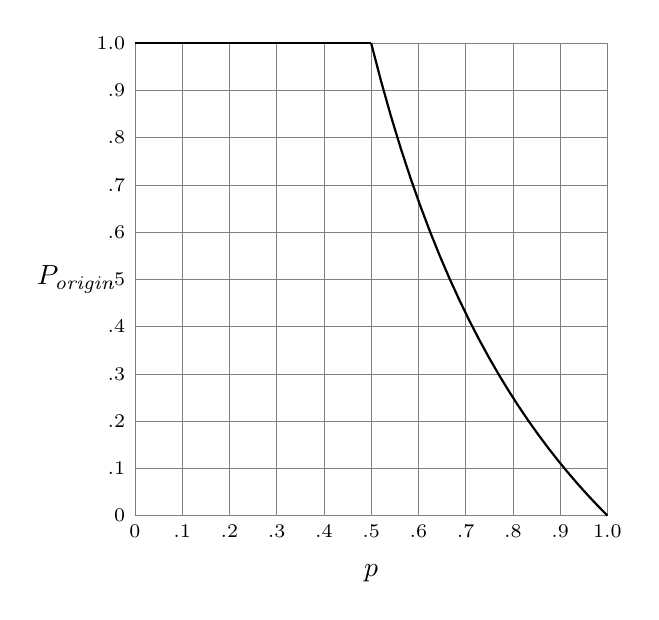
\begin{tikzpicture}[scale=6]
\draw[help lines,step=.1] (0,0) grid (1,1);
\foreach \x in {0,.1,.2,.3,.4,.5,.6,.7,.8,.9,1.0}
  \node[below] at (\x,0) {$\scriptstyle \x$};
\foreach \y in {0,.1,.2,.3,.4,.5,.6,.7,.8,.9,1.0}
  \node[left] at (0,\y) {$\scriptstyle \y$};
\draw[domain=0:.5,thick] plot (\x,1);
\draw[domain=.5:1,thick] plot (\x,{(1-\x)/\x});
\node at (.5,-3.5pt) {$p$};
\node at (-3.5pt,.5) {$P_{\mathit{origin}}$};
\end{tikzpicture}
\caption{Graph of $P_{\mathit{origin}}$}\label{f.walk1}
\end{center}
\end{figure}

$E_{\mathit{origin}}$, the expected duration until the first return to the origin, is infinite for $p\geq 1/2$ while for $p<1/2$ it is:
\[
E_{\mathit{origin}}=\disfrac{1}{q-p}=\disfrac{1}{1-2p}\,.
\]

\subsection{Program structure}

\verb+configuration.py+ contains declarations of variables which are intended to be constant.

\verb+random_walk_plot.py+ contains the functions for plotting a graph of the proportion of simulations until the return to the origin, if the simulation is run for multiple probabilities.

\verb+random_walk.py+ is the main program which obtains the parameters, runs the simulations, prints the output and calls the plotting functions.

\subsection{Running the simulations}

The program runs the simulations in a loop, each time asking the user how to run it. You can run the same simulation again with the saved parameters, enter new parameters, or run a sequence of simulations for a range of probabilities or initial values.

A typical output is as follows:
\begin{verbatim}
Probability = 0.55, step limit   = 1000
Proportion returning to origin   = 0.901
Probability of return to origin  = 0.818
Proportion reaching limit        = 0.099
\end{verbatim}
The results of the simulation are very close to the theoretical probability and expected duration.

Figure~\ref{f.random_walk-01} shows the graph of the proportion of returns to the origin for different values of the probability and for a fixed limit.
\begin{figure}
\begin{center}
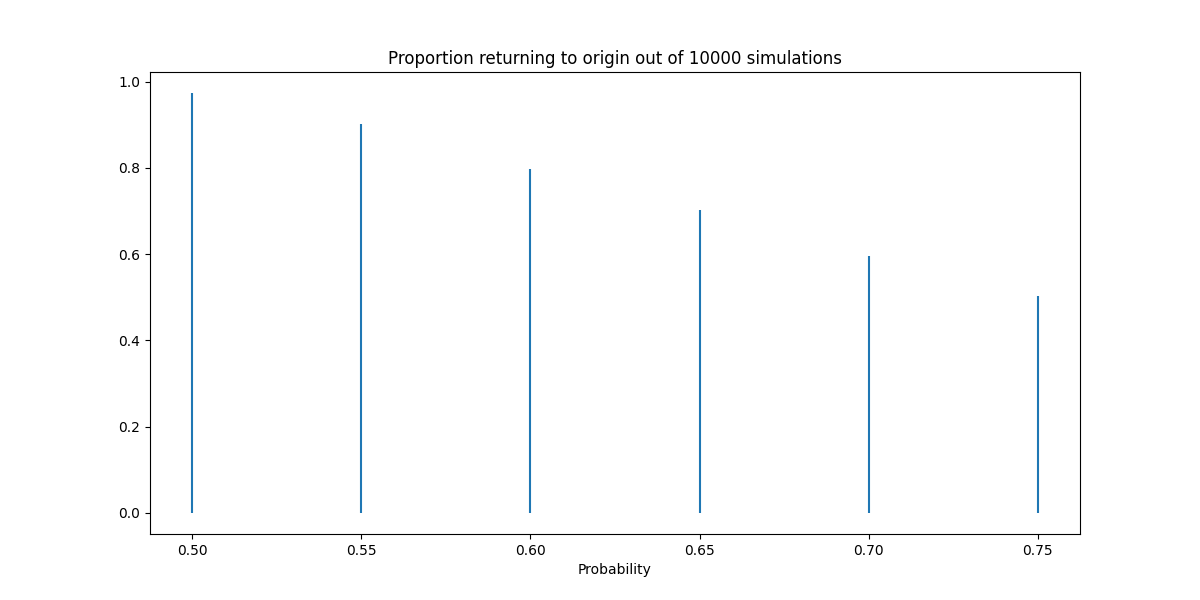
\includegraphics[width=\textwidth]{random_walk-01}
\end{center}
\caption{Graph for a limit of $1000$ steps}\label{f.random_walk-01}
\end{figure}

Figure~\ref{f.random_walk-02} shows the proportion simulations reaching the limit for different values of the limit and for a fixed probability.
\begin{figure}
\begin{center}
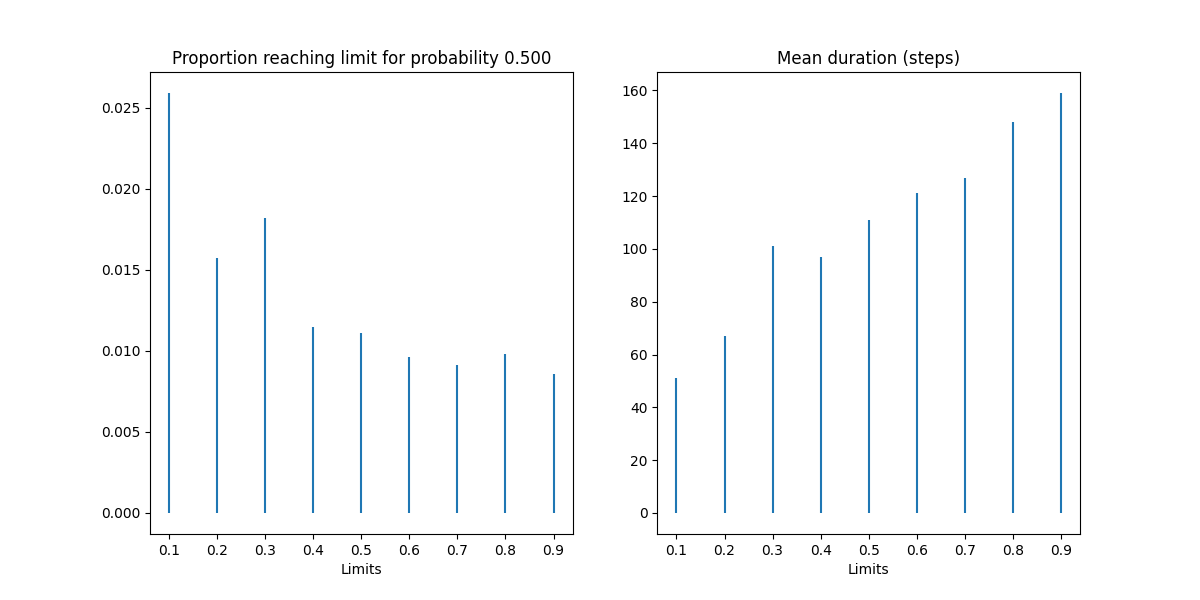
\includegraphics[width=\textwidth]{random_walk-02}
\end{center}
\caption{Proportion of simulations reaching the limit for $p=0.51$}\label{f.random_walk-02}
\end{figure}
